\documentclass[12pt]{article}
\usepackage[left=1cm, right=1cm, top=2cm,bottom=1.5cm]{geometry} 

\usepackage[parfill]{parskip}
\usepackage[utf8]{inputenc}
\usepackage[T2A]{fontenc}
\usepackage[russian]{babel}
\usepackage{enumitem}
\usepackage[normalem]{ulem}
\usepackage{amsfonts, amsmath, amsthm, amssymb, mathtools}
\usepackage{tabularx}
\usepackage{hhline}

\usepackage{accents}
\usepackage{fancyhdr}
\pagestyle{fancy}
\renewcommand{\headrulewidth}{1.5pt}
\renewcommand{\footrulewidth}{1pt}

\usepackage{graphicx}
\usepackage[figurename=Рис.]{caption}
\usepackage{subcaption}
\usepackage{float}

%%Наименование папки откуда забирать изображения
\graphicspath{ {./images/} }

%%Изменение формата для ввода доказательства
\renewcommand{\proofname}{$\square$  \nopunct}
\renewcommand\qedsymbol{$\blacksquare$}

%%Изменение отступа на таблицах
\addto\captionsrussian{%
	\renewcommand{\proofname}{$\square$ \nopunct}%
}
%% Римские цифры
\newcommand{\RN}[1]{%
	\textup{\uppercase\expandafter{\romannumeral#1}}%
}

%% Для удобства записи
\newcommand{\MR}{\mathbb{R}}
\newcommand{\MQ}{\mathbb{Q}}
\newcommand{\MI}{\mathrm{I}}
\newcommand{\MJ}{\mathrm{J}}
\newcommand{\MH}{\mathrm{H}}
\newcommand{\MT}{\mathrm{T}}
\newcommand{\MU}{\mathcal{U}}
\newcommand{\MV}{\mathcal{V}}
\newcommand{\VN}{\varnothing}
\newcommand{\VE}{\varepsilon}

\theoremstyle{definition}
\newtheorem{defn}{Опр:}
\newtheorem{rem}{Rm:}
\newtheorem{prop}{Утв.}
\newtheorem{exrc}{Упр.}
\newtheorem{lemma}{Лемма}
\newtheorem{theorem}{Теорема}
\newtheorem{corollary}{Следствие}

\newenvironment{cusdefn}[1]
{\renewcommand\thedefn{#1}\defn}
{\enddefn}

\DeclareRobustCommand{\divby}{%
	\mathrel{\text{\vbox{\baselineskip.65ex\lineskiplimit0pt\hbox{.}\hbox{.}\hbox{.}}}}%
}
%Короткий минус
\DeclareMathSymbol{\SMN}{\mathbin}{AMSa}{"39}
%Длинная шапка
\newcommand{\overbar}[1]{\mkern 1.5mu\overline{\mkern-1.5mu#1\mkern-1.5mu}\mkern 1.5mu}
%Функция знака
\DeclareMathOperator{\sgn}{sgn}

%Обозначение константы
\DeclareMathOperator{\const}{\text{const}}

%Интеграл в большом формате
\DeclareMathOperator{\dint}{\displaystyle\int}

\newcommand{\smallerrel}[1]{\mathrel{\mathpalette\smallerrelaux{#1}}}
\newcommand{\smallerrelaux}[2]{\raisebox{.1ex}{\scalebox{.75}{$#1#2$}}}

\newcommand{\smallin}{\smallerrel{\in}}
\newcommand{\smallnotin}{\smallerrel{\notin}}

\newcommand*{\medcap}{\mathbin{\scalebox{1.25}{\ensuremath{\cap}}}}%
\newcommand*{\medcup}{\mathbin{\scalebox{1.25}{\ensuremath{\cup}}}}%

%Скалярное произведение
\DeclarePairedDelimiterX{\inner}[2]{\langle}{\rangle}{#1, #2}

%Подпись символов снизу
\newcommand{\ubar}[1]{\underaccent{\bar}{#1}}

\begin{document}
\lhead{Математический анализ - \RN{2}}
\chead{Шапошников С.В.}
\rhead{Лекция - 3}

\section*{$\MR^n$ - линейное, Евклидово, нормированное и метрическое \\пространсво}

\begin{defn}
	$\MR^n = \MR \times \MR \times \dotsc \times \MR = \{\,(x_1, \dotsc, x_n) \mid x_k \in \MR \,\}$ - упорядоченный набор из $n$ чисел.
\end{defn}

\subsection*{Линейное пространство}
\textbf{Операции над наборами}: 
\begin{enumerate}[label={(\arabic*)}]
	\item \textbf{Сложение}: $(x_1, \dotsc, x_n) + (y_1, \dotsc, y_n) = (x_1 + y_n, \dotsc, x_n + y_n)$;
	\item \textbf{Умножение на скаляр} $\alpha \in \MR$: $\alpha{\cdot}(x_1, \dotsc, x_n) = (\alpha x_1, \dotsc, \alpha x_n)$;
\end{enumerate}

С этими операциями $\MR^n$ - \uline{линейное}, \uline{векторное} пространство над $\MR$.

Вектора $e_k = (0,\dotsc,0,\underset{k}{1},0, \dotsc, 0)$ образуют \uline{базис} в $\MR^n$, то есть $\forall x \in \MR^n,\, x = (x_1, \dotsc, x_n)$ единственным образом представляется в виде: $$x = x_1 e_1 + \dotsc + x_n e_n$$ где $x_k$ - координаты вектора $x$.

\subsection*{Евклидово пространство}
На $\MR^n \times \MR^n$ определена функция $x,y \mapsto \inner{x}{y} \in \MR$: 
$$\inner{x}{y} = x_1 y_1 + x_2 y_2 + \dotsc + x_n y_n$$ 
где $x = (x_1, \dotsc, x_n)$, $y = (y_1, \dotsc, y_n)$.

\textbf{Свойства этой функции}:
\begin{enumerate}[label={\arabic*)}]
	\item $\inner{x}{x} \geq 0 \wedge \inner{x}{x} = 0 \Leftrightarrow x = 0$ (неотрицательность);
	\item $\inner{x}{y} = \inner{y}{x}$ (симметричность);
	\item $\inner{\alpha x + \beta z}{y} = \alpha\inner{x}{y} + \beta\inner{z}{y}$ (линейность);
\end{enumerate}

\begin{defn}
	Если на линейном пространстве (над $\MR$) задана функция $\inner{\cdot}{\cdot}$, удовлетворяющая свойствам $1),\, 2)$ и $3)$, то такую функцию называют \uwave{скалярным произведением}, а линейное пространство со скаларням произведением называют \uwave{Евклидовым пространством}.
\end{defn}

\begin{theorem}\textbf{(неравенство Коши-Буняковского-Шварца-Гёльдера)} Справедливо неравенство:
		$$|\inner{x}{y}| \leq \sqrt{\inner{x}{x}}{\cdot}\sqrt{\inner{y}{y}}$$
	причем если верно равенство $\Leftrightarrow x$ и $y$ - линейно зависимы.
\end{theorem}
\begin{proof}
	Пусть $t \in \MR, \, p(t) = \inner{x+ty}{x+ty} = \inner{x}{x} + 2t\inner{x}{y} + t^2\inner{y}{y}$. 
	
	Рассмотрим случай, когда $y = 0 \Rightarrow x,y$ - линейно зависимы $\Rightarrow 0 = 0 + 0 \Rightarrow \inner{x}{0} = \inner{x}{0} + \inner{x}{0} \Rightarrow$ \\
	$\Rightarrow \inner{x}{0} = 0 \Rightarrow |0| = 0 \leq \sqrt{\inner{x}{x}}{\cdot}0 = 0 \Rightarrow$ равенство верно. Далее, считаем $y \neq 0 \Rightarrow \inner{y}{y} \neq 0 \Rightarrow$ имеем квадратный трехчлен.
	
	По свойству $1), \, \forall t, \, p(t) \geq 0 \Rightarrow D \leq 0, \, D = 4\inner{x}{y}^2 - 4\inner{x}{x}\inner{y}{y} \leq 0 \Rightarrow \inner{x}{y}^2 \leq \inner{x}{x}\inner{y}{y} \Rightarrow$ извлекаем корень и получаем требуемое неравенство $|\inner{x}{y}| \leq \sqrt{\inner{x}{x}}{\cdot}\sqrt{\inner{y}{y}}$.
	
	Равенство $\Leftrightarrow D = 0 \Leftrightarrow \exists \, t_0\colon p(t_0) = 0 \Leftrightarrow x + t_0y = 0$, т.е. $x$ и $y$ линейно зависимы.
\end{proof}
\begin{exrc}
	Свести к $\MR^2$ и использовать школьную математику при доказательстве (скорее всего это про площадь параллелограмма). 
\end{exrc}

\subsection*{Нормированное пространство}
Длина или норма вектора $x \in \MR^n$: $\|x\| = \sqrt{\inner{x}{x}}$.

\textbf{Свойства нормы}:
\begin{enumerate}[label={\arabic*)}]
	\setcounter{enumi}{-1}
	\item $\|\cdot\| \colon \MR^n \to [0,+\infty)$; 
	\item $\|x\| = 0 \Leftrightarrow x = 0$;
	\item $\|\alpha x\| = |\alpha|\cdot\|x\|$;
	\item $\|x+y\| \leq \|x\| + \|y\|$ (неравенство треугольника);
	\begin{proof}
		$\|x+y\|^2 = \inner{x +y}{x+y} = \|x\|^2 + 2 \inner{x}{y} + \|y\|^2 \Rightarrow$ по неравенству КБ: $\inner{x}{y} \leq \|x\|{\cdot}\|y\|$. \\ 
		Тогда:
		$$ \|x+y\|^2 = \|x\|^2 + 2\|x\|{\cdot}\|y\| + \|y\|^2 = (\|x\| + \|y\|)^2 \Rightarrow \|x+y\| \leq \|x\| + \|y\|$$
	\end{proof}
\end{enumerate}

\begin{defn}
	Линейное пространство (над $\MR$), на котором задана функция $\|\cdot\|$, удовлетворяющая свойствам $0),\, 1), \, 2)$, и $3)$ называется \uwave{нормированным}, а эта функция называется \uwave{нормой}.
\end{defn}
Бывает ли так, что понятие норма задано, а скалярное произведение - нет? Всегда ли длину вектора можно задать подходящим скалярным произведением? 

Если задана длина вектора, то мы можем выразить скалярное произведение через формулу:
$$\inner{x}{y} = \dfrac{1}{2}\Big( \|x+y\|^2 - \|x\|^2 - \|y\|^2 \Big)$$
Но эта формула далеко не всегда будет задавать скалярное произведение. Есть простой критерий для проверки, что норма будет задавать скалярное произведение.

\begin{exrc}\textbf{(Равенство параллелограмма)}
	\begin{figure}[H]
		\centering
		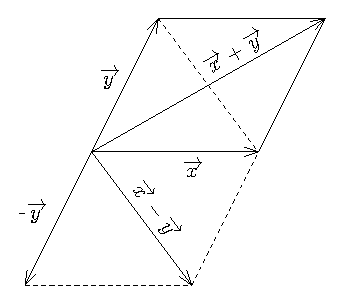
\includegraphics[width=0.35\textwidth]{3_1.eps}
		\caption{Сумма квадратов диагоналей равна сумме квадратов сторон.}
		\label{3_1}
	\end{figure}
Нормированное пространство - Евклидово, тогда и только тогда, когда выполняется равенство параллелограмма $\|x+y\|^2 + \|x-y\|^2 = 2\|x\|^2 + 2\|y\|^2$, доказать равенство при $\|x\| = \sqrt{\inner{x}{x}}$ (необх. условие).
\end{exrc}

Нормированные пространства это более широкий класс пространств, чем Евклидовы. В них есть линейная структура, вектора, длины, но нет углов. В Евклидовом пространстве, есть скалярное произведение $\Rightarrow \cos{\angle{xy}}\dfrac{\inner{x}{y}}{\|x\|{\cdot}\|y\|}\Rightarrow$ есть углы. 

\subsection*{Метрическое пространство}
Функция $\rho(x,y) = \|x-y\|$ обладает следующими свойствами:

\begin{enumerate}[label={\arabic*)}]
	\item $\rho \geq 0, \, \rho(x,y) = 0 \Leftrightarrow x = y$ (неотрицательность);
	\item $\rho(x,y) = \rho(y,x)$ (симметричность);
	\item $\rho(x,y) \leq \rho(x,z) + \rho(z,y)$ (неравенство треугольника);
	\begin{proof}
		$\rho(x,y) = \|x-y\| = \|(x-z) + (z-y)\| \leq \|x-z\| + \|z-y\| = \rho(x,z) + \rho(z,y)$.
	\end{proof}
\end{enumerate}

\begin{defn}
	Если на непустом множестве $X$ определена функция $\rho \colon X \times X \to [0, +\infty)$, удовлетворяющая свойствам $1),\,2)$ и $3)$, то такая функция называется \uwave{метрикой}, а пара $(X,\rho)$ \uwave{метрическим пространством}.
\end{defn}

\textbf{Переходы}: Евклидово пространство $\Rightarrow$ нормированное пространство $\Rightarrow$ метрическое пространство - это упрощение структуры. В метрическом пространстве у нас есть только множество и ``линейка'', чтобы замерять расстояния между точками. Далее мы будем расширяться от понятия метрического пространства к Евклидову.

\textbf{Примеры метрических пространств}:
\begin{enumerate}[label={(\arabic*)}]
	\item $\MR^n, \, \rho(x,y) = \sqrt{ \displaystyle \sum\limits_{k=1}^{n}(x_k - y_k)^2}$  - метрическое пространство (разбирается в школе). Такакя метрика называется \uwave{Евклидовой};
	\item $X \neq \VN, \, \rho(x,y) = \begin{cases} 1, & x \neq y \\ 0, & x = y \end{cases} $, свойства $1)$ и $2)$ будут выполнены, проверим $3)$:
	\begin{proof}
		$\rho(x,y) \leq \rho(x,z) + \rho(z,y)$, в худшем случае слева будет $1$, при $x \neq y$, если $\rho(x,z) = 0 \Rightarrow x = z$, если $\rho(z,y) = 0 \Rightarrow y = z \Rightarrow x = z = y \Rightarrow \rho(x,y) = 0$, что будет протворечием, если $x \neq y \Rightarrow$ неравенство треугольника выполняется.
	\end{proof}
	Такая метрика называется \uwave{дискретной};
	
	\item $\MR, \, \rho(x,y) = |f(x) - f(y)|$, где $f$ - некоторая функция. $2), \, 3)$ - выполняются. Свойство $1)$ выполняется, когда
	$\rho(x,y) = 0 \Leftrightarrow f(x) = f(y) \Rightarrow$ функция должна быть инъективной;
	
	\item $\MR^n, \, \rho(x,y) = \displaystyle \sum\limits_{k=1}^{n}|x_k - y_k|$ - метрическое пространство;
	
	\item $\MR^n, \, \rho(x,y) = \max\limits_{1 \leq k \leq n}|x_k - y_k|$, свойства $1)$ и $2)$ будут выполнены, проверим $3)$:
	\begin{proof}
		$\forall k =\overline{1,n}, \, |x_k - y_k| \leq |x_k - z_k| + |z_k - y_k| \Rightarrow |x_k - y_k| \leq \max\limits_{1 \leq k \leq n}|x_k - z_k| + \max\limits_{1 \leq k \leq n}|z_k - y_k| \Rightarrow$ \\
		$\Rightarrow  \max\limits_{1 \leq k \leq n}|x_k - y_k| \leq \max\limits_{1 \leq k \leq n}|x_k - z_k| + \max\limits_{1 \leq k \leq n}|z_k - y_k|$ так как справа от $k$ ничего не зависело.
	\end{proof}
	Таким образом это тоже метрическое пространство;
	
	\item $\{0,1\}^n = \{\,(\underbrace{0,1,0,0,1,1,0, \dotsc}_{n}) \,\}, \, \rho(x,y) = \displaystyle \sum\limits_{k=1}^{n}|x_k - y_k|$ - метрическое пространство. Такая метрика называется \uwave{расстоянием Хемминга}, она указывает в скольких ``битах'' было различий.
	
	\item $X \neq \VN, \, B(X) = \{\, f \mid f\colon X \to \MR, \, f \text{ - ограничена}\,\}, \, \rho(f,g) = \sup\limits_{x}|f(x) - g(x)|,\, \forall f,g \in B(X)$,\\  $B(X)$ - множество всех ограниченных функций из $X$ в $\MR$. Если взять $X = \{1,2, \dotsc, n\}$, то это будет частный случай - пример $(5)$. Свойства $1), \, 2)$ - очевидны, остается доказать неравенство треугольника:
	\begin{proof}
		$\forall x \in X,\, |f(x) - g(x)| \leq |f(x) - z(x)| + |z(x) - y(x)| \Rightarrow  \forall x \in X,\, |f(x) - g(x)| \leq \sup\limits_{x}|f(x) - z(x)| +$\\
		$ + \sup\limits_{x}|z(x) - y(x)| \Rightarrow \sup\limits_{x}|f(x) - g(x)| \leq \sup\limits_{x}|f(x) - z(x)| + \sup\limits_{x}|z(x) - y(x)|$, так как справа от $x$ ничего не зависело.
	\end{proof} 
\end{enumerate}

\begin{defn}
	\uwave{Открытым шаром} с центром в точке $a$ и радиусом $r$ называется $B(a,r) = \{\, x \mid \rho(a,x) < r \, \}$.
\end{defn}
\begin{defn}
	\uwave{Замкнутым шаром} с центром в точке $a$ и радиусом $r$ называется $\overline{B}(a,r) = \{\, x \mid \rho(a,x) \leq r \, \}$.
\end{defn}

\textbf{Пример}: $\MR^2,\, \rho(x,y) = |x_1 - y_1| + |x_2 - y_2|$, нарисуем как выглядит $B(0,1) = \{\,(x_1,x_2) \mid |x_1| + |x_2| < 1 \,\}$:
\begin{figure}[H]
	\centering
	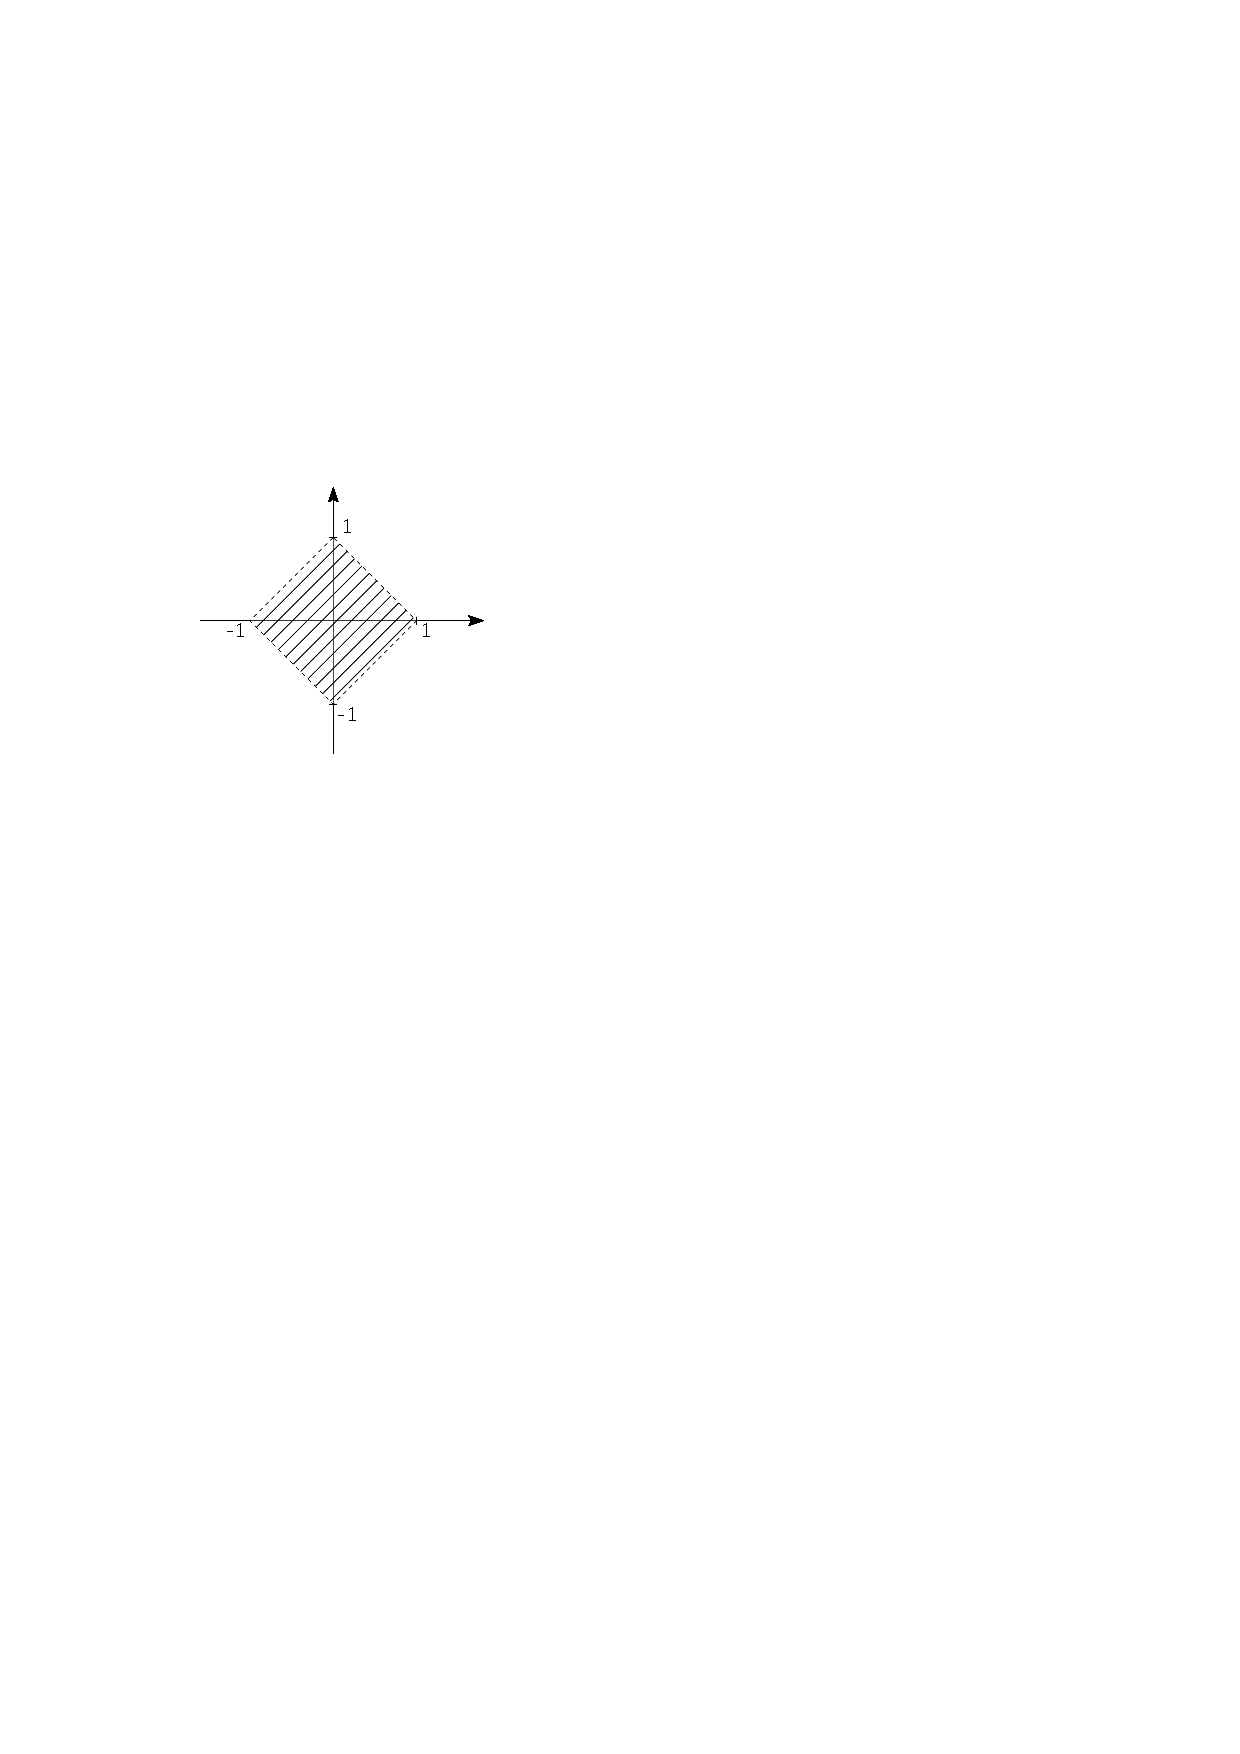
\includegraphics[width=0.25\textwidth]{3_2.png}
	\caption{Пример открытого шара $B(0,1) = \{\,(x_1,x_2) \mid |x_1| + |x_2| < 1 \,\}$.}
	\label{3_2}
\end{figure}

Может оказаться, что шар с большим радиусом лежит строго внутри шара малого радиуса.

\textbf{Пример}: Возьмем прямоугольный треугольник $\triangle ABC$. В качестве метрического пространства возьмем его вершины $X = \{\,A, B, C \,\}$. Построим два шара $B(C,r) \wedge B(A,R) \colon R > r \Rightarrow$ 
$$B(C,r) =  \{\,A, B, C \,\} \supsetneq B(A,R) =  \{\,A, C \,\}$$
\begin{figure}[H]
	\centering
	\includegraphics[width=0.25\textwidth]{3_3.eps}
	\caption{Пример шара большего радиуса, содержащегося внутри шара меньшего радиуса.}
	\label{3_3}
\end{figure}

\end{document}
